\documentclass[11pt,reqno,final]{amsart}

\pdfcompresslevel=0
\pdfobjcompresslevel=0

\usepackage[dvipsnames]{xcolor}% adds colors
\usepackage{amsmath, amsthm}% {amsfonts, amssymb}

% New Characters
\usepackage[latin1]{inputenc}%
\usepackage[T1]{fontenc}

\usepackage{MnSymbol}
\usepackage[normalem]{ulem}% underlining

\usepackage[theoremfont, largesc]{newpxtext} % different text,math font
\usepackage{newpxmath}

\makeatletter
\DeclareMathRadical{\sqrtsign}{symbols}{112}{largesymbols}{112}
% \let\sqrt=\undefined
% \DeclareRobustCommand\sqrt{\@ifnextchar[\@sqrt{\mathpalette\@x@sqrt}]}
% \def\@x@sqrt#1#2{%
%  \setbox\z@\hbox{$\m@th#1\sqrtsign{\mkern1mu #2}$}
%  \mkern3mu\box\z@}
\makeatother




% Page Typesetting
\usepackage[final]{microtype}
\usepackage{relsize}
\usepackage[margin=1in]{geometry}
\usepackage{framed}
\usepackage{tikz}
\usepackage{setspace}

\usepackage{hyperref}
\hypersetup{
  final,
  pdftitle={Math 135 - Trig Limits},
  pdfauthor={Bonventre}, 
  linktoc=page,
  pagebackref,
  colorlinks=true,
  citecolor=PineGreen,
  linkcolor=PineGreen,
  linkbordercolor=PineGreen,
}


% Internal References

\usepackage[inline,shortlabels]{enumitem}

% \numberwithin{equation}{section} 
\numberwithin{figure}{section}

\usepackage[nameinlink,capitalise,noabbrev]{cleveref}

\crefname{equation}{}{} % get \cref to behave as \eqref

% \theoremstyle{plain} % bold name, italic text
\newtheorem{theorem}[equation]{Theorem}%
\newtheorem*{theorem*}{Theorem}%
\newtheorem{lemma}[equation]{Lemma}%
\newtheorem{proposition}[equation]{Proposition}%
\newtheorem{corollary}[equation]{Corollary}%
\newtheorem{conjecture}[equation]{Conjecture}%
\newtheorem*{conjecture*}{Conjecture}%
\newtheorem{claim}[equation]{Claim}%
\newtheorem{question}{Question}

\theoremstyle{definition} % bold name, plain text
\newtheorem{definition}[equation]{Definition}%
\newtheorem*{definition*}{Definition}%
\newtheorem{example}[equation]{Example}%
\newtheorem*{example*}{Example}%
\newtheorem{remark}[equation]{Remark}%
\newtheorem{notation}[equation]{Notation}%
\newtheorem{convention}[equation]{Convention}%
\newtheorem{assumption}[equation]{Assumption}%
\newtheorem{exercise}[question]{Exercise}

% ---------- macros
\newcommand{\set}[1]{\left\{#1\right\}}%
\newcommand{\sets}[2]{\left\{ #1 \;|\; #2\right\}}%
\newcommand{\longto}{\longrightarrow}%
\newcommand{\into}{\hookrightarrow}%
\newcommand{\onto}{\twoheadrightarrow}%

\usepackage{harpoon}
\newcommand{\vect}[1]{\text{\overrightharp{\ensuremath{#1}}}}

\newcommand{\del}{\partial}%

\newcommand{\ki}{\chi}
\newcommand{\ksi}{\xi}
\newcommand{\Ksi}{\Xi}

\newcommand{\dlim}{\displaystyle\lim}

% %%%%%%%%%%%%%%%%%%%%%%%%%%%%%%%%%%%%%%%%%%%%%%%%%%%%%%%%%%%%%%%%%%%%%%%%%%%%%%%%%%%%%%%%%%%%%%%%%%%%

\begin{document}
\onehalfspacing

\begin{center}
        \textbf{\Large Math 135, Calculus 1, Fall 2020}\\[10pt]
        {\large 10-02: Trig limits and the Squeeze Theorem}
\end{center}

\thispagestyle{empty}

\renewcommand{\thesection}{\Alph{section}}

\vspace{-1pt}
\section{Solving limits algebraically}

Last class, we reviewed the number of ways we can evaluate the limit $\dlim_{x \to a}f(x)$:
\begin{itemize}
\item If we know the function $f(x)$ is continuous at $x = a$, then the limit is simply $f(a)$.
\item If we have the \textit{graph} of the function $f$, we can visually determine the limit.
\item We can perform numerical calculations.
\item We can use algebra.
\end{itemize}

The algebraic route is particularly useful if ``evaluation'' yields an \textbf{indeterminant form}:
\[
        \dfrac{0}{0}, \quad  \dfrac{\infty}{\infty}, \quad  \infty \cdot 0, \quad \infty - \infty
\]

Some techniques we saw on 09-28 to deal with these:
\begin{itemize}
\item \textbf{Limits as} $\mathbf{x \to \boldsymbol{\pm\infty \colon}}$ only the \textit{highest powers of $x$ matter}. The rest we can ignore.
\item $\mathbf{0/0:}$ Try canceling a common factor from both the numerator and the denominator.\\
        \textit{This may require you to factor polynomials, or expand functions.}
\item \textbf{Square roots and} $\mathbf{0/0:}$ If we have square roots in the numerator or denominator,
        try multiplying the top and bottom by the \textit{conjugate}.
\item $\boldsymbol{\infty - \infty \colon}$ Try combining the two terms and simplifying.
\end{itemize}

\section{The Squeeze Theorem}

Today, we will use a new technique for when the above fail.

\begin{theorem}[The Squeeze Theorem]
        Suppose that $f(x) \leq g(x) \leq h(x)$ when $x$ is near $a$ (except possibly at $x=a$),
        and that
        \[
                \dlim_{x \to a} f(x) = \lim_{x \to a} h(x) = L.
        \]
        Then $\dlim_{x \to a} g(x) = L$.
\end{theorem}
\textit{That is, if $g(x)$ is bounded above and below by two functions that limit on the same value as $x \to a$, then
  $g(x)$ also limits on that same value.}

\begin{center}
        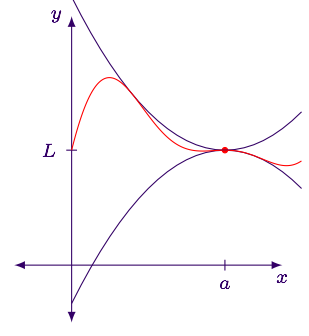
\includegraphics[width=2in]{10-02P_squeeze.png}
\end{center}

\newpage

\begin{example}
        Using the Squeeze Theorem, let's show that $\dlim_{x \to 0} x^2 \sin(1/x) = 0$.
        Evaluating, we get $0 \cdot DNE$, which is unhelpful.
        However, we know the range of $\sin \theta$ is just $[-1,1]$, so this gives us bounds for $\sin(1/x)$: 
        \[
                -1 \leq \sin(1/x) \leq 1
        \]
        Multiplying through by $x^2>0$ does not change the inequality signs, so we get
        \[
                -x^2 \leq x^2 \sin(1/x) \leq x^2 
        \]
        But now $\dlim_{x \to 0} -x^2 = \dlim_{x \to 0} x^2 = 0$, so the limit of the bounded function
        $\dlim_{x \to 0} x^2 \sin(1/x) = 0$.        
\end{example}

\begin{exercise}
        Use the Squeeze Theorem to compute $\dlim_{x \to \infty} \dfrac{\sin x}{x}$.
        \vfill
\end{exercise}

Two important trig limits are the following:
\begin{framed}
        \[
                \dlim_{x \to 0} \dfrac{\sin x}{x} = 1 \qquad \mbox{and} \qquad \dlim_{x \to 0} \dfrac{1 - \cos x}{x} = 0.
        \]
\end{framed}

\begin{example}
        To prove the first one, we use the fact that
        \[
                \cos x \leq \dfrac{\sin x}{x} \leq 1 \qquad \mbox{for $\frac{-\pi}{2} < x < \frac{\pi}{2}$}
        \]
        \begin{center}
                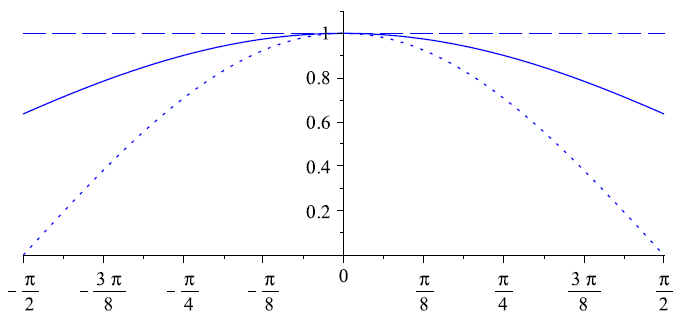
\includegraphics[width=4in]{10-02P_sinxx.png}
        \end{center}
        \begin{itemize}
        \item Solid line: $y = \dfrac{\sin x}{x}$
        \item Dashed line: $y = 1$
        \item Dotted line: $y = \cos x$
        \end{itemize}
        Since $\dlim_{x \to 0} \cos x = \dlim_{x \to 0} 1 = 1$, the Squeeze Theorem implies $\dlim_{x \to 0} \dfrac{\sin x}{x} = 1$, as desired.
\end{example}

\newpage

\begin{exercise}
        Using the limit $\dlim_{x \to 0} \dfrac{\sin x}{x} = 1$, show that $\dlim_{x \to 0} \dfrac{1 - \cos x}{x} = 0$.\\
        \textit{Hint: Multiply the top and bottom by $1 + \cos x$; simplify; and then break the fraction into the product of two fractions, one of which is $\dfrac{\sin x}{x}$.}
        \vfill        
\end{exercise}

\begin{exercise}
        Evaluate $\dlim_{x \to 0} \dfrac{\sin^2 x}{x^2}$.\\
        \textit{Hint: the limit of a product equals the product of the limits.}
        \vfill
\end{exercise}

\begin{exercise}
        Evaluate $\dlim_{t \to 0} \dfrac{\sin(7t)}{t}$.\\
        \textit{Hint: Make the substitution $x = 7t$. If $t \to 0$, what is $x$ approaching?
          Use this substitution to rewrite the limit using only the variable $x$ in a way so that $\dfrac{\sin x}{x}$ is present.}
        \vfill
\end{exercise}

\end{document}
